\chapter{Background}\label{chap:background}
% This chapter will perform a breath-first explanation on the contents related
% with the thesis. The extension of the contents explained here can be seen as
% monotone function over the number of missing pages to attain the requirements.
%
% Some topics are indeed important as its the case of factor graphs.
% Others like:
%  - classification (SVM, multi-class, kernel-trick),
%  - features (SIFT, GIST),
%  - Basic Bayes theory and probabilistic review
% are included for fun of the reader in case it inquires himself how to deal
% with the low-levels features we propose using.
%
% ---
% PS: This is the chapter that will be used to fill with unnecessary crap
% in case they really annoy me with the number of pages. Every other chapter
% will strive to be really required and be a masterpiece.
%

\section{Classification}
\subsection{Recognition and Categorization}
\subsection{Support Vector Machines}
\Glspl{SVM} where introduced by \cite{cortes1995support} and can be seen as
discriminative linear based classifier. They are based on a strong mathematical
foundation and have powerful generalization capabilities. In their original form
\gls{SVM} separates two classes of points in an hyper-space with a
\emph{maximal margin hyperplane}~(\autoref{fig:svm-sample}).

Later they were extended to deal with noisy data by using \emph{soft margins}.
And to handle non-linear spaces as seen on \autoref{sec:kernel-trick}.
Although they only allow for two class-classification several methods have been
proposed to build multi-class classifiers based on binary classifiers as seen on
\autoref{sec:multiclass-classifiers}.

\begin{figure}[h]
\begin{center}
% TODO: get a decent picture to illustrate SVMs
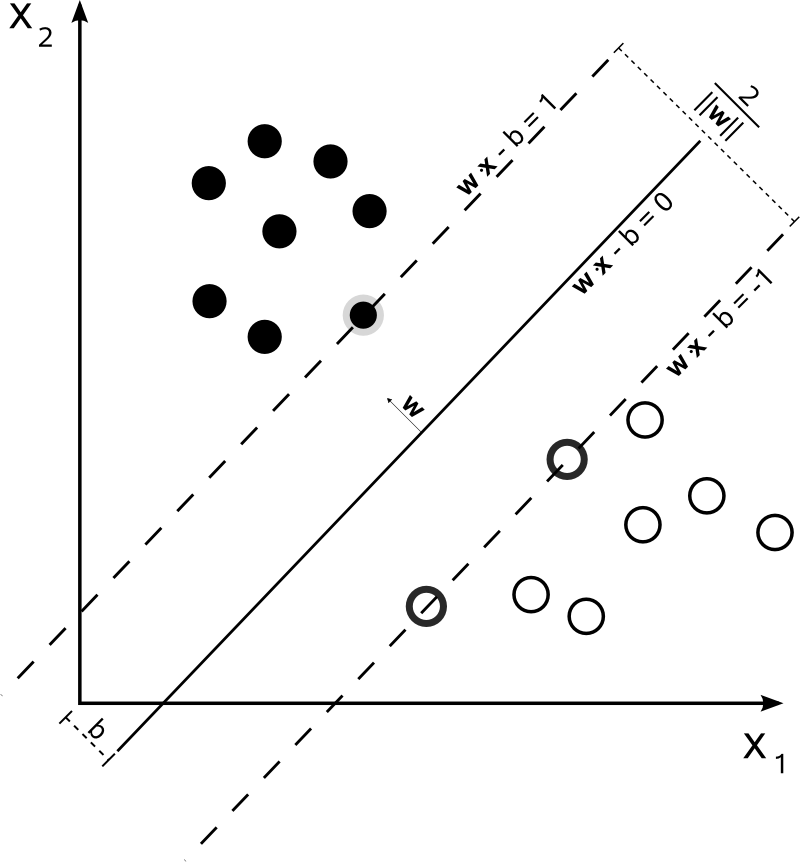
\includegraphics[width=0.4\textwidth]{figures/Svm_max_sep_hyperplane_with_margin}
\end{center}
\caption{{SVM} separating two class of points by a
         \emph{maximal margin hyperplane}. The hyperplane can be described by
         the collection of support vectors and associated weights, marked in the
         image as sample points with large borders.}
\label{fig:svm-sample}
\end{figure}

They have been used in several classification and recognition problems and are
in fact a standard across machine learning techniques. Their efficiency, exact
training results and generalization made their suitable for many tasks. Such as
text categorization, digit-recognition, spam-classification.
They have also been extensively used in visual place classification.


\subsection{Multi-Class Classification}
\label{sec:multiclass-classifiers}
\Glspl{SVM} were designed as two-class classifier. And so they need to be
adapted for using in multi-class problems. The most common usage is to design
multi-class classifiers recurring at the usage of multiple two-class classifiers
and methods for combining them. The most typical approaches for a multi-class
classification on $c$ classes using \glspl{SVM} are:

\begin{description}
\item[One Against All] - in this method $c$ distinct classifiers are trained to
distinguish any class of the remaining ones. The output of all those classifiers
(distance to the separating hyperplane) is then used to categorize the output.
The most common approach is to pick the class with the largest hyperplane
distance. Other variations exists as is the case of using the minimal distance
to the average classification distance of each class~\citep{pronobis2007confidence}.

\item[One Against One] - in this method $c*(c-1)/2$ classifiers are trained to
distinguish between each pair of classes. The final decision is based on the
output of all those classifiers being common to use a majority vote strategy.
\end{description}

\subsection{Kernel-Trick}
\label{sec:kernel-trick}
\gls{SVM} in their basic form are only able to handle linear spaces.
Nonetheless the classes are most of the time not linearly separable in the input
space. Although there might exists a transformation $\phi$ from the original
space into a space $H$ where the input becomes linearly separable.

The Kernel trick allows to extend the \gls{SVM} definition to work on such space
$H$ without ever performing an implicit transformation between spaces. Being
enough for that to have a Kernel function defining an inner-product inside such
space: $K(x_i, x_j) = \phi(x_i)\cdot\phi(x_j)$.
In that sense a Kernel function can be seen as a function that calculates some
similarity measure between two inputs.

Several kernel functions have been proposed being the most commonly used:

\begin{description}
\item[Polynomial Kernel] - $K(x, y) = (x \cdot y + p)^d$
\item[Radial Basis Function] - $K(x, y) = e^{-\gamma\|x - y \|^2}$
\item[Histogram intersection] - $K(x, y) = e^{-\gamma \chi^2(x,y)}$, where
$\chi^2(x,y) = \sum_{i=1}^{N}\frac{(x_i-y_i)}{x_i+y_i}$ introduced by
\cite{barla2003histogram} allows to compute histogram similarity.
\item[Matching Kernels] - mimic matching similarity and are used when each
sample is represented as a set of features~\citep{boughorbel2005intermediate}.
\end{description}

\section{Features}
A feature is a piece of information which is expected to reveal information for
solving a specific task. In that sense features are task-dependant and they will
yield different performance based on the type of task they are applied to.

A wanted property on features is its repeatability under similar conditions for
the problem in hand. This is: they should be stable and invariant across
unwanted types of transformations and noise. For example a visual feature for
object detection should be present even if the target object was translated,
scaled, rotated, the light-conditions have changed or even if the object is
partially occluded.

Extracting features with those properties allows to greatly reduce the size of
input by removing unwanted noise and useless information from the captured data.
Turning the classification problem easier, more reliable and more efficient.

Often several and different types of features need to be extracted. It has been
reported by \cite{pronobis2010ijrr} that using multiple features provides a
great benefit in the context of place classification.
And \cite{quattoni2009recognizing} has showed that different types have
different impact in indoor scene recognition based on the type of scene
matching. Namely was seen that some room-categories are more likely to be
recognized by the presence of some objects and others by it generic appearance.

In the context of robotics, sensors such as cameras, laser scans are used to
sense the surrounding environment, and features can be extracted from all those.
Nonetheless as described in \autoref{sec:visual-motivation} the visual sensor is
incredibly rich and most of our features will come from it.

Visual features can be seen as belonging to two categories:
\emph{local features} and \emph{global features}.
\emph{Local features} describe fine grain properties of a part of image.
For example the existence of specific corner or an edge. \Gls{SIFT}
(\autoref{sec:sift}) is an example of such feature and has been proven useful
for matching points between images and subsequence extension to object detection.

\emph{Global features} such as \gls{CRFH} (\autoref{sec:crfh}) or
{gist}~(\autoref{sec:gist}) try to describe the whole image. Either by
statistical analysis of features over all the image or by a structured
distribution of textures findable in the image.

\subsection{Local Features}
\label{sec:local-features}

\subsubsection{SIFT}
\label{sec:sift}
The detection of interesting points has been studied for several years and is
the base of several computer vision problems solution. It allows to perform
point matching which can be used in several areas from image stitching,
3D reconstruction, video tracking, object detection, etc\dots

The most used method was presented by \cite{lowe1999object}. And its based on
building a feature vector for each image. Each of those features is based on
\emph{interesting points} detected by detecting maxima and minima of a
difference of Gaussian functions applied in a scale-space.
The scale space is used to provide scale invariant detection. Gaussian functions
are used as they are the only way to model a linear scale-space.
Each interesting point is then described by a container that is rotation
invariant.

By seeing an object as a set of features points, index and matching is then
performed by a high-dimensional search on a database of know objects. After
matching objects can be verified for geometric coherence between features.
\Gls{SVM} classifiers can also be trained to detect objects based on this type
of local features by using \emph{Matching kernels} (\autoref{sec:kernel-trick}).

\begin{figure}[h]
    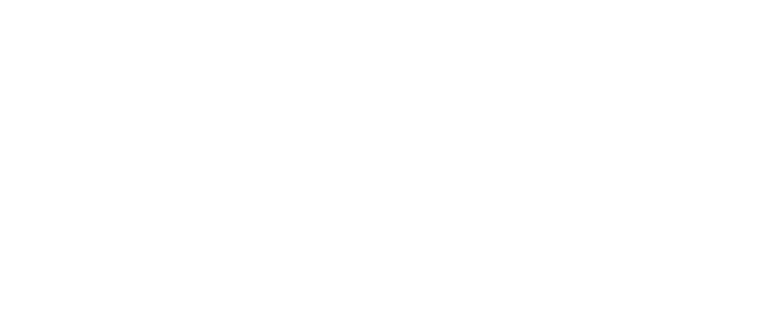
\includegraphics[width=\textwidth]{figures/sift/sift.pdf}
    \caption{{SIFT} and other local features have been proven useful in object
             detection.}
\end{figure}


\subsection{Global Features}

\subsubsection{Gist of a Scene}
\label{sec:gist}
\cite{oliva2006building} argue that fast scene recognition does not need to be
built on top of object recognition but can be analyzed by scene-centered
mechanisms.
They defend that position by pointing out behaviours on human vision:
when provided with a glance of a shot a person can identify the meaning of that
given shot or "gist of a scene" without remembering specific details.

\begin{figure}[h]
\center
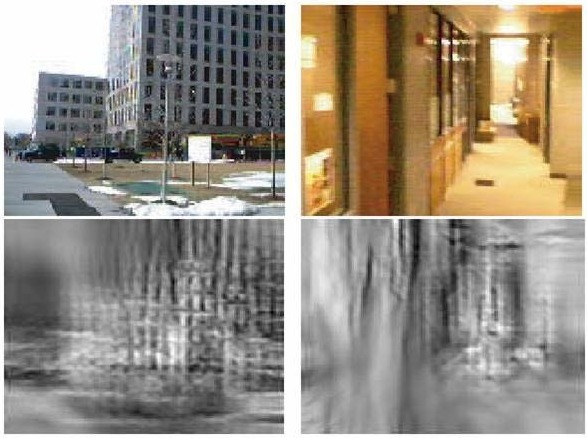
\includegraphics[width=0.60\textwidth]{figures/gist.jpg}
\caption{An illustration of the gist of an image. Top row: original image I;
         bottom row: noise image J for which gist(I) = gist(J). We see that the
         gist captures the dominant textural features of the overall image, and
         their coarse spatial layout~\citep{murphy2006object}.}
\end{figure}


\subsubsection{{CRFH} - Composed Receptive Field Histograms}
\label{sec:crfh}\label{sec:global-features}
Composed Receptive Field Histograms are a multidimensional statistical
representation of the occurrence of several image descriptors applied to an
image. They can be seen as an high-dimension histogram where each cell records
how many pixels of the image have the cell response for the applied descriptors.
Such high-dimensional histogram is expected to be able to better global
information contained in the image by capturing several properties of the image
as well the relations between them.


\begin{figure}[h]
\begin{center}
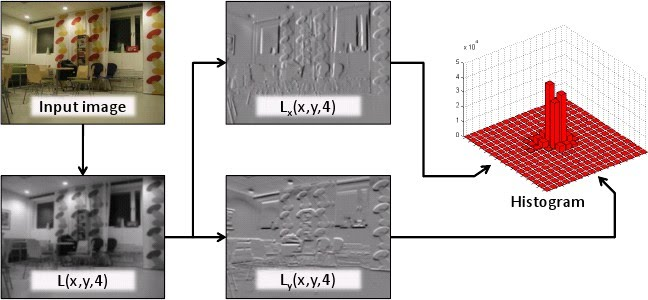
\includegraphics[width=1\textwidth]{figures/crfh_model.jpg}
\end{center}
\caption{A two dimensional histogram of the image built out from two image
         descriptors: $Lx$ and $Ly$. First-order Gaussian derivatives of image
         luminance in horizontal and vertical direction applied at a scale 4.}
\end{figure}

Several type of image descriptors can be applied.
For example Gaussian derivatives (such as $L_x$, $L_y$, $L_{xx}$, $L_{yy}$) are
partial derivatives of the image luminance after applying a Gaussian filter of a
given scale ($\sigma$) on the image. Gradient magnitude descriptors
(such as $|\nabla L|$) can also be used as a rotation invariant descriptor.


One of the problems of high-dimensional histograms is the memory and
computationally complexity needed to handle them.
\cite{linde2004object} suggested using a sparse form to represent those by
storing only the non-zero-cells in an array structure.

Multidimensional histograms have proven to be useful in the context of object
recognition~\citep{schiele1996object}. And have also been previously used in
the context of visual place classification~\cite{pronobis2010ijrr}.
\emph{Histogram intersection kernels} (\autoref{sec:kernel-trick}) can be used
to train classifiers based on this feature.

\subsection{Laser Features}


%%%%%%%%%%%%%%%%%%%%%%%%%%%%%%%%%%%%%%%%%%%%%%%%%%
% Important sections of this chapter begin here.
%%%%%%%%%%%%%%%%%%%%%%%%%%%%%%%%%%%%%%%%%%%%%%%%%%
\clearpage
\section{Probability Theory}
\subsection{Bayes Theorem}

\subsection{Categorical and Multinomial Distribution}

\section{Probabilistic Graphical Models}
\label{sec:graphical-models}
% THIS IS ALL JUNK TEXT COPIED
Graphical models usage can be tracked back to earlies 1920 but they only become
popular in mid-eighties when researchers started to use \emph{Bayesian Networks}
to model expert systems~\citep{borgelt2002graphical}.

They serve as a better tool to model \emph{random variables}
(nodes on the graph) and their probabilities as they model the conditional
dependence between variables (edges on the graph). Important to note that here
\emph{random variables} does not denotes a truly random variable but one that is
unknown by the system and is conditioned by other variables/evidences.

This type of graphs provide a generative model where the probability of any
given scenario can be determined. As opposed to non-generative models where a
given probability can only be calculated if certain data is given.
This means when a graphical model is learned, it can be used to generate new
samples from the learned distribution.

They have been successfully used in several machine-learning task such as:
information extraction, speech recognition, computer vision.
They are also useful due to their ability to deal with semantic (high-level)
features~\citep{boutell2006factor} and ability to represent properties of the
reality they try to model.

Two main types of graphical models have been used: Bayesian Networks which model
directed edges between variables and Markov Random Fields where variables are
connected by a potential but no special direction is given to edges.

An important property of these graphs is the \emph{Markov-blanket} of a node.
For a given variable $a$, a \emph{Markov-blanket} is a set of variables in the
surroundings of $a$ that when given the value of $a$ becomes independent of the
rest of the graph~\citep{pearl1988probabilistic}.
On non-directional graphs it is directly determined by the nodes connected to $a$.
This allows the usage of graph algorithms such as \emph{min-cut} to quickly
determine most likely scenarios. In the case of directed edges a node blanket is
also influenced by the direction of the edges and a more complex schemes need to
be used.

As \cite{lauritzen2002chain} points this two types of models can be represented
as a \emph{chain graph} where both directed and undirected edges can co-exist.
Though this generalization is hard to implement due to mis-understandings on the
concepts the graph-models use.

Another useful interpretation of graphical-models are \emph{factor graphs}.
Those are able to handle both \emph{Bayesian Networks} and
\emph{Markov Random Fields}. Under this interpretation a graph is seen as a
bipartite graph that connects variables with factors that influence
them~\citep{bishop2006pattern}.
This gives a very useful framework to develop belief propagation on them by
seeing a message-passing mechanism between nodes. Belief propagation is used to
calculate marginal-probabilities.

\begin{figure}[ht]
    \begin{minipage}[b]{0.3\linewidth}
        \centering
        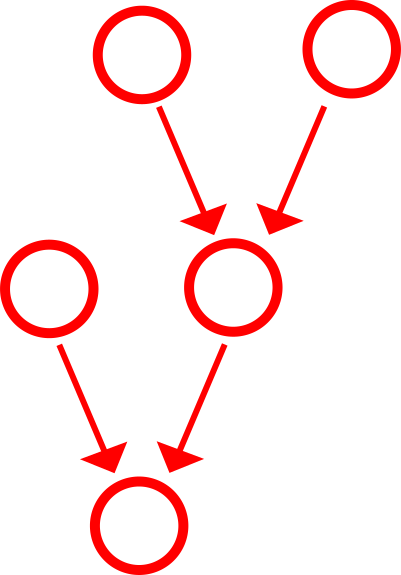
\includegraphics[width=0.8\textwidth]{figures/graphical-models/BayesNet.pdf}
        \caption{Bayes Networks}
    \end{minipage}
    \hspace{0.5cm}
    \begin{minipage}[b]{0.3\linewidth}
        \centering
        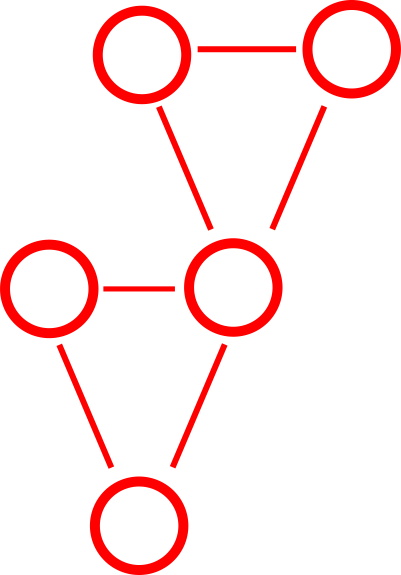
\includegraphics[width=0.8\textwidth]{figures/graphical-models/MarkovRandomField.pdf}
        \caption{Markov Random Field}
    \end{minipage}
    \hspace{0.5cm}
    \begin{minipage}[b]{0.3\linewidth}
        \centering
        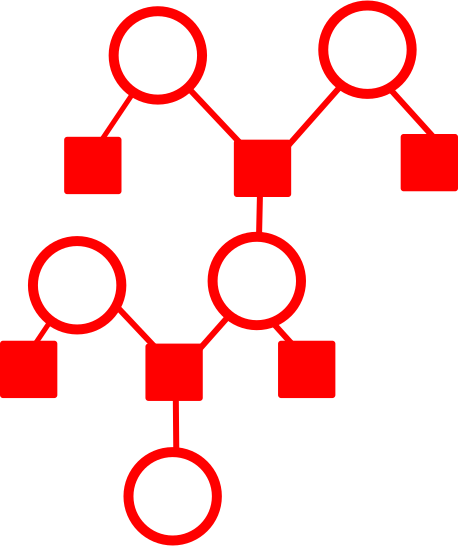
\includegraphics[width=\textwidth]{figures/graphical-models/FactorGraph.pdf}
        \caption{Factor Graph}
    \end{minipage}
\end{figure}

\subsection{Factor Graphs}
A \emph{factor graph} is a bipartite graph connecting two sets of nodes $X_G$ and $F_G$
representing random variables and factors.
Each factor is described by function $\phi$ dependent only on the variables $x_\phi$
to which the factor is connected.
Thus, a factor graph can be seen as a description of probability density function obtained
by a product of all the factors. In order to represent the probability,
a normalization factor needs to be introduced, resulting in the following equation:

\begin{equation}
P_G(x) = \frac{1}{Z}\prod_{\phi \in F_G}{\phi(x_{\phi})},\qquad
Z = \sum_{X_G}\prod_{\phi \in F_G}{\phi(x_{\phi})}
\end{equation}


More often we are only interested in a marginal of the probability distribution.

\begin{equation}
M_G(x) = \frac{1}{Z}\sum_{X_G \backslash x}{\prod_{\phi \in F_G}{\phi(x_{\phi})}}
\end{equation}

\subsection{Inference Engines}
Exact Inference and Approximate Inference methods

\section{Principle of Maximum Entropy}
\label{sec:max-entropy}
The principle of maximum entropy states that given a set of distributions that
are coherent with the acquired knowledge, the one which maximizes entropy should
be picked.

In the case of non-available information this is the uniform distributions.
In cases where we only know the mean and standard deviation a normal
distribution shall be picked, etc\dots

% In case we expand in some finding structure in graphs maybe the following will
% be useful
\section{Label Propagation, Min-Cuts}



